% Chapter Template

\chapter{Ensayos y Resultados} % Main chapter title
\label{Chapter4}

En este capítulo se presentan las pruebas realizadas para validar el correcto funcionamiento del sistema implementado. Se incluyen pruebas funcionales de cada bloque en particular y de todo el sistema integrado.

\section{Pruebas funcionales}

A medida que se desarrollaron los diferentes módulos del firmware del sistema, se llevaron a cabo las correspondientes pruebas en cada uno de ellos, para validar que funcionaban de la manera esperada antes de ser integrados con otras partes del sistema. Todas las pruebas fueron realizadas manualmente.

Los bloques a probar se pueden dividir en tres grupos: la comunicación por WiFi, la comunicación utilizando BLE y la comunicación con el electrodoméstico.

\subsection{Comunicación WiFi}

La comunicación por WiFi es la parte del sistema más compleja y la que por lo tanto requiere pruebas más exhaustivas de sus diferentes funcionalidades.

Independientemente de la aplicación que se le vaya a dar, el primer paso es lograr conectarse exitosamente a una red WiFi. Esta fue la primera prueba realizada, configurando a mano las credenciales de la red inalámbrica y verificando por consola que se conecte correctamente, como se puede ver en la figura \ref{fig:output_wifi_connection}. En ella, se ve que se inició la conexión y luego se registró el evento en el que el microcontrolador obtuvo una dirección IP y por lo tanto se conectó con éxito.

\begin{figure}[h]
\centering
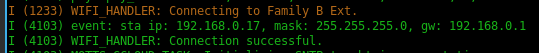
\includegraphics[width=\textwidth]{./Figures/output_wifi_connection.png}
\caption{Salida por consola del microcontrolador al conectarse a una red WiFi.}
\label{fig:output_wifi_connection}
\end{figure}

Una vez llegado a este punto, es posible continuar con las pruebas asociadas a la comunicación con el usuario del electrodoméstico, mediante una interfaz de usuario, y con el fabricante, enviando información hacia Google Cloud.

\subsubsection{Comunicación con el usuario}

A los fines de contar con algún mecanismo que permita enviar comandos desde Internet de parte del usuario del electrodoméstico, se recurrió a diferentes plataformas web IoT configurables ya existentes.

Para las pruebas de envío y recepción mediante los protocolos HTTP y HTTPS, se utilizó ThingSpeak \citep{thingspeak}. Esta plataforma permite recibir información desde el microcontrolador, almacenarla y graficarla. Además, permite enviar comandos desde la página hacia el microcontrolador. Si bien ThingSpeak ofrece una librería para interactuar con la plataforma, en este caso se utilizaron directamente las direcciones indicadas en su documentación para enviar HTTP \emph{requests} desde las tareas de transmisión y recepción WiFi que se ejecutan en el microcontrolador. De esta forma, por un lado se enviaron comandos desde ThingSpeak y se observó por consola que el microcontrolador los recibía correctamente. Por otro lado se enviaron datos periódicamente hacia ThingSpeak y se los graficó, verificando que tenían los valores esperados.

Para demostrar la versatilidad del módulo desarrollado, se decidió utilizar una plataforma IoT diferente para probar la comunicación utilizando MQTT. Por eso se utilizó Adafruit IO \citep{adafruit}, plataforma que permite crear tableros o \emph{dashboards} personalizados para comunicarse con sistemas embebidos. La figura \ref{fig:adafruit_dashboard} muestra la interfaz desarrollada, en la que se puede ver que se tienen diferentes botones para mandar comandos determinados, un historial de comandos enviados, un cuadro mostrando el estado del electrodoméstico (\emph{slave}) y un cuadro con el último comando enviado.

\begin{figure}[h]
\centering
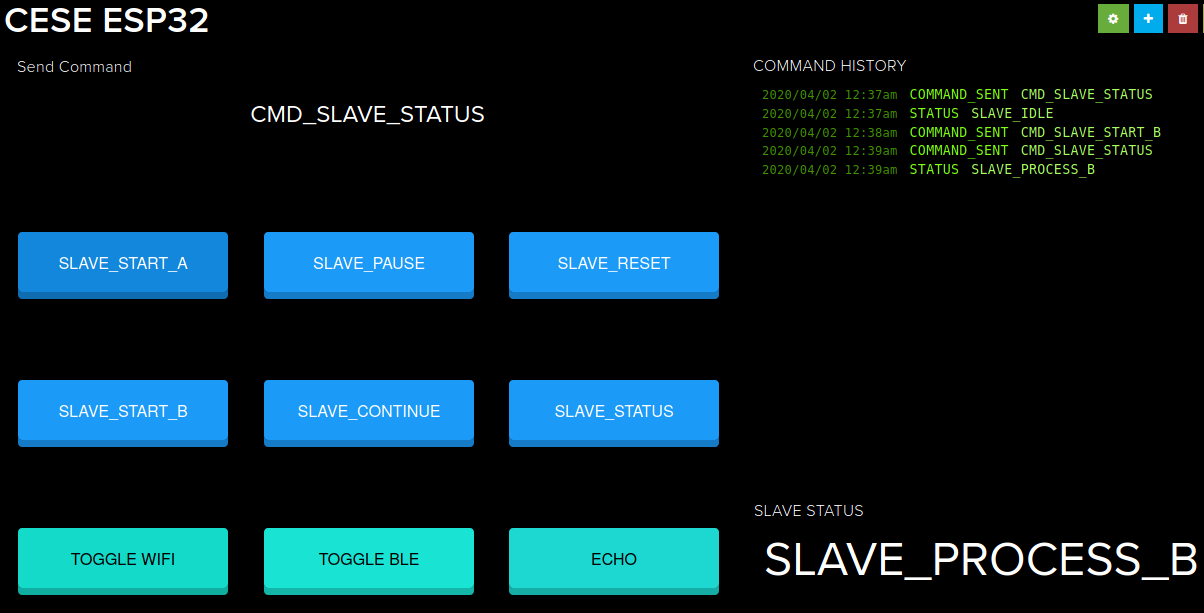
\includegraphics[width=\textwidth]{./Figures/adafruit_dashboard.png}
\caption{Interfaz de usuario creada en Adafruit IO.}
\label{fig:adafruit_dashboard}
\end{figure}

En el historial de comandos se puede observar que se envió un comando para conocer el estado del electrodoméstico (CMD\_SLAVE\_STATUS) y se recibió de vuelta el estado actual (SLAVE\_IDLE, es decir inactivo sin ejecutar ninguna acción). Luego se envió un comando para iniciar un proceso en el electrodoméstico (CMD\_SLAVE\_PROCESS\_B), y al preguntar nuevamente por el estado, se obtuvo que se encontraba ejecutando la acción iniciada con el comando anterior.

Desde el punto de vista del firmware, en la figura \ref{fig:output_mqtt_connection} se observa cómo van ocurriendo los diferentes eventos asociados a MQTT (descriptos en la sección \ref{sec:wifi_com}). 

\begin{figure}[h]
\centering
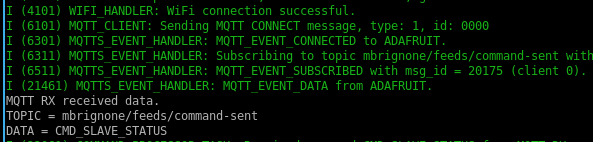
\includegraphics[width=\textwidth]{./Figures/output_mqtt_connection.png}
\caption{Eventos disparados en el microcontrolador por la comunicación utilizando MQTT.}
\label{fig:output_mqtt_connection}
\end{figure}

Primero se espera a que el \emph{driver} WiFi indique que la conexión ya está habilitada, y luego se envía la orden de conectarse al \emph{broker} MQTT, disparándose a continuación el evento MQTT\_EVENT\_CONNECTED, el cual indica que la conexión al \emph{broker} fue exitosa. 

Para detectar los comandos enviados por el usuario, el cliente se suscribe al \emph{topic} correspondiente, lo cual dispara el evento MQTT\_EVENT\_SUBSCRIBED.

Finalmente, se dispara el evento MQTT\_EVENT\_DATA indicando que hay un dato nuevo en el \emph{topic} al cual el microcontrolador se encuentra suscrito, y se puede ver que el dato recibido se corresponde al comando enviado desde Adafruit.

\subsubsection{Comunicación con el fabricante}

La comunicación con el fabricante consiste en el envío de datos desde el microcontrolador hacia Google Cloud utilizando el protocolo MQTT. Para ello primero el dispositivo debe conectarse al \emph{broker} de Google Cloud y autenticarse mediante un JSON Web Token, tal como se explicó en la sección \ref{sec:google_cloud}. Este proceso se puede observar en la figura \ref{fig:output_gcloud_connection}, donde se aprecia cómo se generó el JWT, para lo cual se obtuvo el tiempo actual mediante el protocolo SNTP, y luego se conectó a Google Cloud.

\begin{figure}[h]
\centering
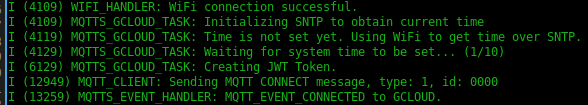
\includegraphics[width=\textwidth]{./Figures/output_gcloud_connection.png}
\caption{Conexión del microcontrolador a Google Cloud por MQTT.}
\label{fig:output_gcloud_connection}
\end{figure}

Una vez conectado al \emph{broker}, se enviaron algunos mensajes y luego se revisó el registro de eventos (\emph{logs}) de Google Cloud para verificar que la comunicación fue exitosa. Esto se ilustra en la figura \ref{fig:gcloud_log}, en la que se ve que primero se produce la conexión de un dispositivo, luego la publicación de dos mensajes (con intervalos de 30 segundos entre ellos) y finalmente la desconexión del dispositivo. Cabe mencionar que en el registro se cuenta con mucha más información que la mostrada en la figura \ref{fig:gcloud_log}, pero se la omite por simplicidad.

\begin{figure}[h]
\centering
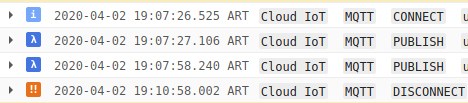
\includegraphics[width=\textwidth]{./Figures/gcloud_log.png}
\caption{Registro de eventos MQTT en Google Cloud.}
\label{fig:gcloud_log}
\end{figure}

\subsubsection{Servidor web}

Para probar el funcionamiento del servidor web, es necesario conectarse a la red local que el propio módulo genera, cuyo nombre es ESP32\_AP. Una vez conectado, es posible acceder al servidor ingresando a una dirección IP específica desde cualquier navegador.

La interfaz del servidor web es sumamente sencilla, y solamente consiste en un formulario para ingresar las credenciales de la red WiFi a la cual se desea conectar, tal como se observa en la figura \ref{fig:web_server_interface}.

\begin{figure}[h]
\centering
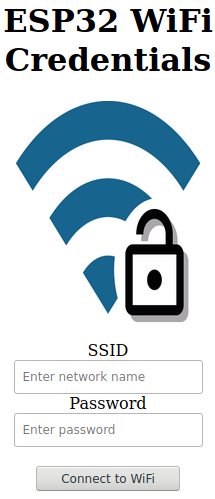
\includegraphics[scale=0.5]{./Figures/web_server_interface.png}
\caption{Interfaz del servidor web que se ejecuta en el módulo.}
\label{fig:web_server_interface}
\end{figure}

Desde el punto de vista del firmware, en la figura \ref{fig:output_web_server} se observan los diferentes eventos que ocurrieron al conectarse a la red local del módulo funcionando como punto de acceso.

Primero se detectó la conexión de un nuevo cliente (\emph{station}) al punto de acceso. Debido a que el objetivo del servidor web es permitir configurar o modificar las credenciales WiFi, se observa cómo el módulo se desconectó en ese momento de la red WiFi a la que se encontraba conectado. Luego el servidor web detectó que se envió el formulario, mostrando por consola las credenciales de la red ingresada. Finalmente el firmware desconectó automáticamente al cliente que estaba en el servidor web y procedió a conectarse a la nueva red.

\begin{figure}[h]
\centering
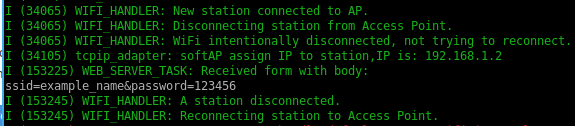
\includegraphics[width=\textwidth]{./Figures/output_web_server.png}
\caption{Salida por consola del microcontrolador durante la configuración de las credenciales de la red WiFi.}
\label{fig:output_web_server}
\end{figure}

\subsection{Comunicación BLE}

Para probar el funcionamiento de la comunicación por Bluetooth Low Energy, se utilizó en un celular la aplicación móvil \emph{nRF Connect}, que ofrece un poderoso conjunto de herramientas para comunicarse con dispositivos BLE. Entre ellas se encuentra la posibilidad de descubrir servicios/características y realizar operaciones de lectura/escritura sobre ellas.

Al iniciar el módulo, el WiFi se encuentra encendido por defecto, y por lo tanto el BLE está apagado, ya que ambos no pueden coexistir en simultáneo. Por ello como primera prueba se envió un comando para encender el BLE, para verificar que el WiFi se desactiva automáticamente y el proceso de BLE se inicializa correctamente. En la figura \ref{fig:ble_init} se observa cómo se inicia el controlador Bluetooth y luego se disparan cuatro eventos asociados al servidor BLE (como se explicó en la sección \ref{sec:ble_com}). Estos eventos indican que se registró la aplicación, que se creó e inició un servicio, y que se agregó una característica a dicho servicio.

\begin{figure}[h]
\centering
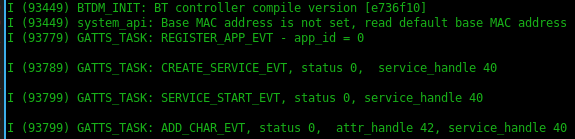
\includegraphics[width=\textwidth]{./Figures/ble_init.png}
\caption{Inicialización de la interfaz BLE en el módulo.}
\label{fig:ble_init}
\end{figure}

Una vez inicializada la comunicación BLE, es posible descubrir el módulo utilizando la aplicación \emph{nRF Connect}, como se observa en la figura \ref{fig:nrf_discover_esp32}.

\begin{figure}[h]
\centering
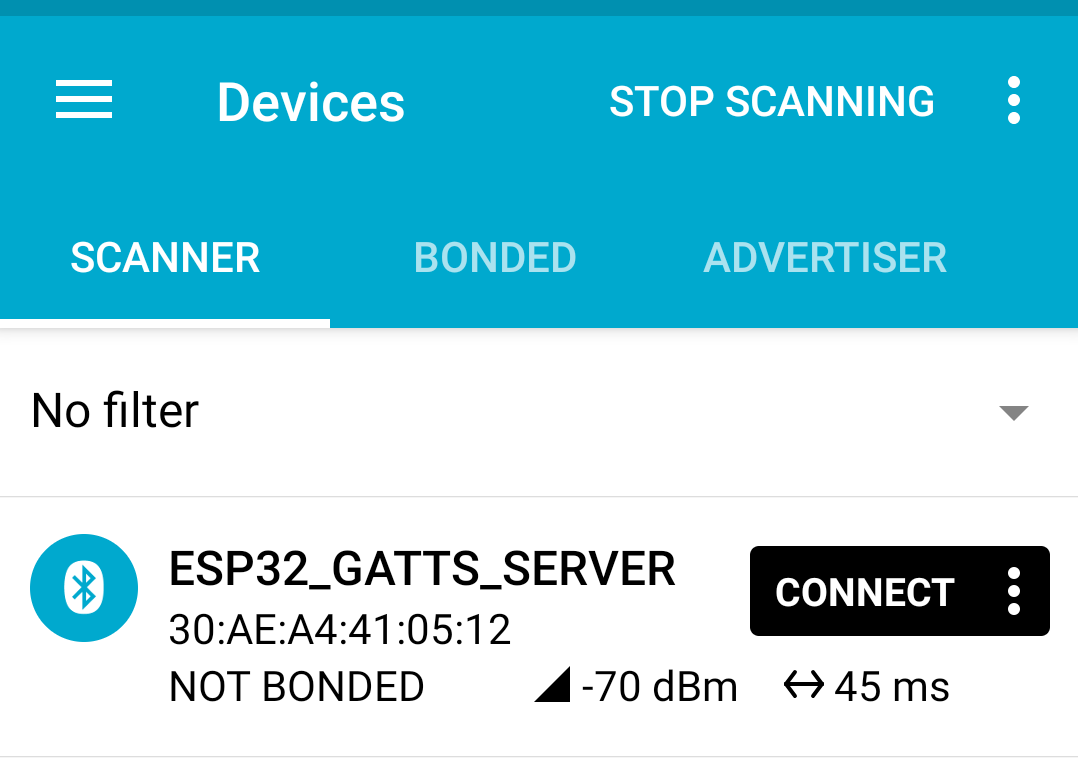
\includegraphics[scale=0.16]{./Figures/nrf_discover_esp32.png}
\caption{Servidor BLE del módulo visible en la aplicación móvil nRF Connect.}
\label{fig:nrf_discover_esp32}
\end{figure}

Al establecer una conexión con el módulo desde la aplicación, se puede acceder a sus servicios y características. Esto queda en evidencia en la figura \ref{fig:nrf_char_esp32}, en la que se ve el servicio con su correspondiente característica, los cuales fueron previamente configurados en el firmware del módulo. Ambos figuran como \emph{unknown} debido a que los identificadores no se corresponden con ningún valor predefinido por el \emph{Bluetooth Special Interest Group}.

\begin{figure}[h]
\centering
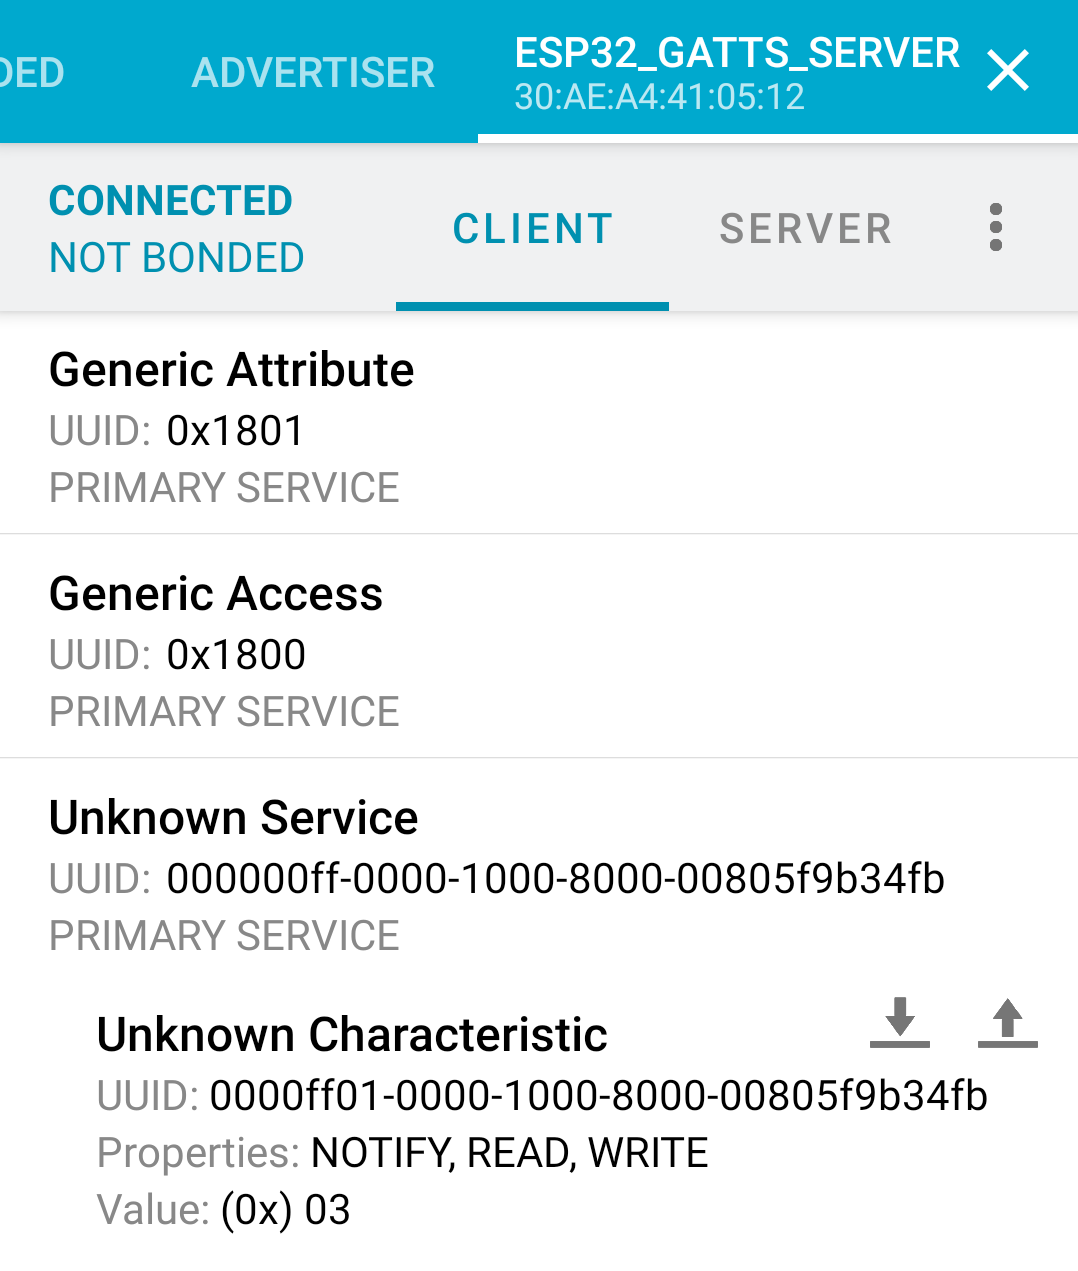
\includegraphics[scale=0.20]{./Figures/nrf_char_esp32.png}
\caption{Servicio con su correspondiente característica, vistos en la aplicación móvil nRF Connect.}
\label{fig:nrf_char_esp32}
\end{figure}

Los símbolos de flecha ubicados a la derecha de la característica permiten leer o escribir un valor, disparando así en el firmware los eventos correspondientes (figura \ref{fig:output_ble_event}, con tres operaciones de lectura y una de escritura con valor 0x01).

\begin{figure}[h]
\centering
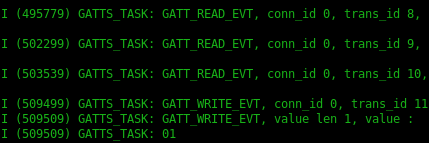
\includegraphics[width=\textwidth]{./Figures/output_ble_event.png}
\caption{Eventos disparados en el firmware ante operaciones de lectura y escritura de una característica BLE.}
\label{fig:output_ble_event}
\end{figure}


\subsection{Comunicación con electrodoméstico}
\label{sec:pruebas_com_serie}

Para probar la comunicación serie por I2C con el electrodoméstico, emulado por otro microcontrolador ESP32, se conectaron las respectivas interfaces I2C como se muestra en la figura \ref{fig:esp32_connection}. Adicionalmente se interconectaron los terminales de masa de ambos microcontroladores.

\begin{figure}[h]
\centering
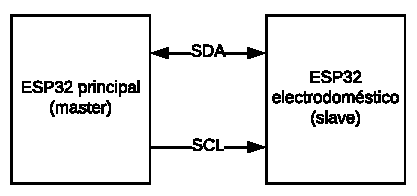
\includegraphics[scale=1.0]{./Figures/esp32_connection.pdf}
\caption{Conexión de las interfaces I2C de los microcontroladores.}
\label{fig:esp32_connection}
\end{figure}

También fue necesario ejecutar un firmware más sencillo en el microcontrolador auxiliar, con una tarea principal que periódicamente lee la información que llega por I2C y en función de ello actualiza una máquina de estados, la cual representa el estado en el que se encuentra el electrodoméstico en un momento dado.

De esta forma fue posible verificar el funcionamiento de la comunicación serie, al enviar un comando desde el módulo principal hacia el microcontrolador que emula el electrodoméstico, y comprobando que se reciben correctamente. Estas pruebas se llevaron a cabo utilizando el módulo UART para enviar comandos al bloque procesador de comandos, que se encarga de transmitir la orden al electrodoméstico (a través de la tarea encargada de la comunicación con él).

En la figura \ref{fig:output_i2c_master} se observa la salida por consola de las pruebas efectuadas.

\begin{figure}[h]
\centering
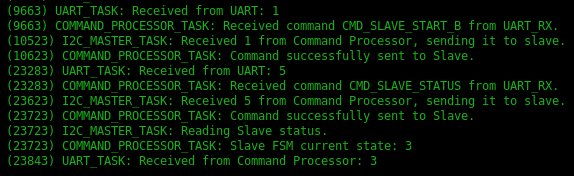
\includegraphics[width=\textwidth]{./Figures/output_master_i2c.png}
\caption{Salida por consola del módulo al comunicarse con el electrodoméstico.}
\label{fig:output_i2c_master}
\end{figure}

Primero se envió por UART el comando 1, que llegó al procesador de comandos y se detectó que se corresponde con una acción a disparar en el electrodoméstico, por lo que se lo envió al módulo encargado de la comunicación serie (I2C\_MASTER\_TASK). Este último envió el comando al otro microcontrolador (el esclavo o \emph{slave} I2C), indicándole al procesador de comandos que pudo hacerlo exitosamente.

Luego se envió por UART el comando 5, el cual indica que se desea conocer el estado del electrodoméstico. La primera parte es idéntica al caso del comando anterior, pero posteriormente la tarea de comunicación serie lee el estado del otro microcontrolador y se lo comunica al procesador de comandos. En este caso se recibió un 3, que se corresponde con el estado SLAVE\_PROCESS\_B.

En la figura \ref{fig:output_slave_i2c} se aprecia lo que ocurrió desde el punto de vista del microcontrolador esclavo que emula al electrodoméstico, pudiéndose ver que el comportamiento es consistente con las órdenes enviadas por el módulo principal. Primero se recibió el comando 1 y la máquina de estados pasó al estado SLAVE\_PROCESS\_B. Luego se recibió el comando 5 y se envió por I2C el estado actual en el que se encontraba.


\begin{figure}[h]
\centering
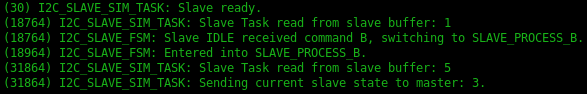
\includegraphics[width=\textwidth]{./Figures/output_slave_i2c.png}
\caption{Salida por consola del microcontrolador que emula al electrodoméstico, al recibir comandos desde el microcontrolador principal.}
\label{fig:output_slave_i2c}
\end{figure}

\section{Integración del sistema}

Para probar el funcionamiento general del sistema, todas las tareas asociadas a los diferentes módulos de firmware deben estar ejecutándose en simultáneo. Esto permite verificar el flujo completo, desde el envío de un comando por parte del usuario (usando la plataforma web) hasta la ejecución de la acción correspondiente en el electrodoméstico (emulado por otro microcontrolador).

En la figura \ref{fig:output_init} se observa cómo se inicializan las diferentes conexiones del sistema. Primero se produce la conexión a la red WiFi y comienza a ejecutarse el servidor web. Una vez conectado a la red, se producen las conexiones con los \emph{brokers} MQTT: Adafruit (para la interacción con el usuario) y Google Cloud (para el envío de datos al fabricante), que requiere también la generación del JSON Web Token (JWT).

\begin{figure}[h]
\centering
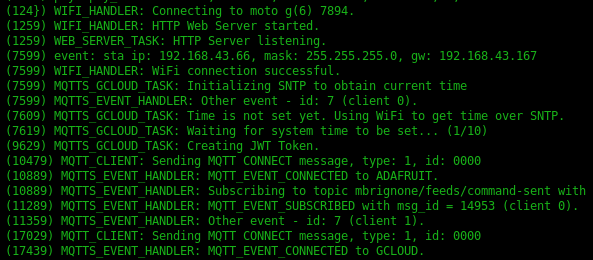
\includegraphics[width=\textwidth]{./Figures/output_init.png}
\caption{Salida por consola al inicializar todos los módulos del sistema.}
\label{fig:output_init}
\end{figure}

A continuación (figura \ref{fig:output_gcloud_mqtt}) se puede observar cómo se envía periódicamente a Google Cloud la información de estado del electrodoméstico. Para ello, la tarea de Google Cloud le envía el comando CMD\_SLAVE\_STATUS al procesador de comandos para obtener el estado del electrodoméstico, de la misma forma que lo haría el usuario. El procesador de comandos obtiene el estado de la forma explicada en la sección \ref{sec:pruebas_com_serie} y se lo pasa de regreso a la tarea de Google Cloud, que se encarga de publicarlo. Se puede observar también el formato JSON que se utiliza para enviar la información de interés.

\begin{figure}[h]
\centering
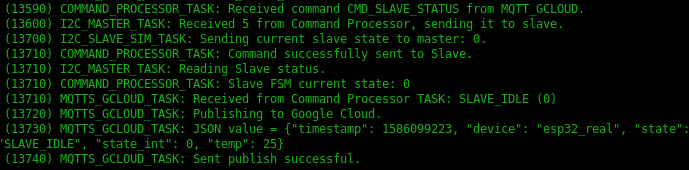
\includegraphics[width=\textwidth]{./Figures/output_gcloud_mqtt_json.png}
\caption{Salida por consola al momento de enviar datos a Google Cloud.}
\label{fig:output_gcloud_mqtt}
\end{figure}

La figura \ref{fig:output_rx_command} muestra la salida por consola cuando el usuario envía un comando desde la plataforma web, evidenciando un comportamiento muy similar al caso anterior.

\begin{figure}[h]
\centering
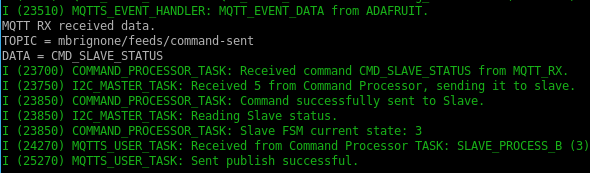
\includegraphics[width=\textwidth]{./Figures/output_rx_command.png}
\caption{Salida por consola al momento de recibir un comando del usuario por WiFi.}
\label{fig:output_rx_command}
\end{figure}

Una prueba importante al integrar el sistema consiste en verificar la correcta transición entre la conexión WiFi y la conexión BLE. Esto requiere especial cuidado ya que al activar una, automáticamente se desactiva la otra, deshabilitando también todas las conexiones que hubiese en ese momento. Posteriormente, al volver a activarse la primera, se deben restablecer todas las conexiones satisfactoriamente.

Al iniciar el sistema, la conexión WiFi se encuentra habilitada, por lo que desde la plataforma WiFi se envía el comando CMD\_BLE para habilitar el BLE, desencadenando los eventos de la figura \ref{fig:output_enable_ble}.

\begin{figure}[h]
\centering
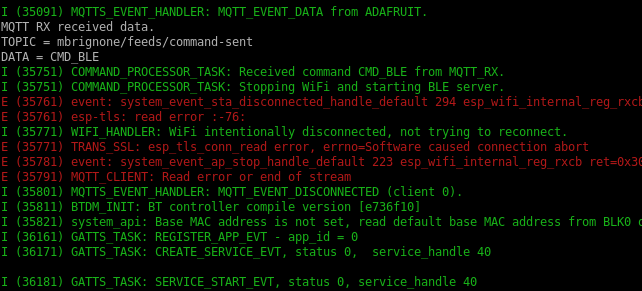
\includegraphics[width=\textwidth]{./Figures/output_enable_ble.png}
\caption{Salida por consola al habilitar la conectividad BLE, estando previamente conectado por WiFi.}
\label{fig:output_enable_ble}
\end{figure}

Al recibir el comando, se desactiva la conexión WiFi y se inicializa el servidor BLE, disparando los eventos correspondientes para crear e iniciar el servicio.

El \emph{event handler} del \emph{driver} WiFi detecta que se desconectó intencionalmente de la red, por lo que no intenta volver conectarse automáticamente. El WiFi se deshabilita de manera asincrónica, por lo que se interrumpen todas las conexiones que estaban activas y por ello aparecen errores de conexión en la salida por consola (en rojo y etiquetados con la letra E en la figura \ref{fig:output_enable_ble}).

Se debe notar que mientras se encuentra habilitada la conectividad BLE, y por lo tanto deshabilitado el WiFi, no es posible enviar información de estado a Google Cloud.

En este punto se puede verificar la transición en el sentido inverso, es decir pasando de BLE a WiFi. Para ello se manda el comando CMD\_WIFI por Bluetooth, lo cual desactiva el BLE y habilita el WiFi, desencadenando los eventos de la figura \ref{fig:output_enable_wifi}. Se puede observar cómo se produce otra vez la inicialización de la conexión WiFi y del servidor web, para luego proceder a realizar exitosamente la conexión por MQTT a ambos \emph{brokers} (Adafruit para el usuario y Google Cloud para el fabricante). Nuevamente hay errores de conexión en el medio debido a la transición, pero luego se conecta correctamente.

\begin{figure}[h]
\centering
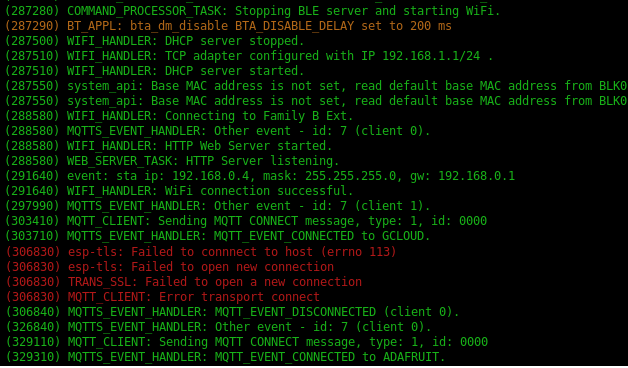
\includegraphics[width=\textwidth]{./Figures/output_enable_wifi.png}
\caption{Salida por consola al habilitar la conectividad WiFi, estando previamente conectado por BLE.}
\label{fig:output_enable_wifi}
\end{figure}

\subsection{Visualización de datos en Google Cloud Platform}

El último aspecto que resta mostrar es el procesamiento y visualización de datos en Google Cloud Platform. La información enviada por el dispositivo a Google Cloud se puede acceder desde múltiples servicios dentro de la plataforma.

Por un lado, como ya se mostró en la figura \ref{fig:gcloud_log}, es posible ver los \emph{logs} y conocer con precisión en qué momento se produjeron las conexiones, envío de datos y desconexiones de los distintos dispositivos. Además, en ese punto se puede filtrar con facilidad para obtener solamente los errores que hayan ocurrido en la comunicación.

Por otro lado, toda la información publicada se puede ver en el \emph{topic} correspondiente creado en el servicio de Cloud Pub/Sub. Para ello se debe crear una suscripción al tema en cuestión y hacer una solicitud de los datos, obteniendo como resultado lo que se observa en la figura \ref{fig:gcloug_topic}.

\begin{figure}[h]
\centering
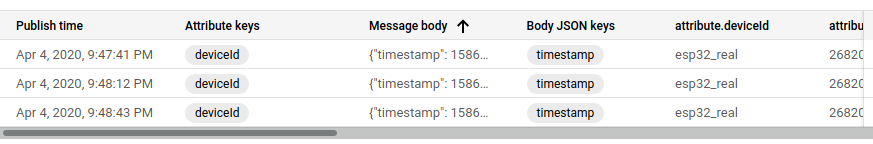
\includegraphics[width=\textwidth]{./Figures/gcloug_topic.png}
\caption{Datos publicados en un \emph{topic} de Cloud Pub/Sub por el microcontrolador.}
\label{fig:gcloug_topic}
\end{figure}

Sin embargo, la mejor forma de analizar y procesar los datos crudos es a través de la base de datos en el servicio Big Query. Gracias a la arquitectura de la figura \ref{fig:google_cloud_diagram}, todos los datos publicados en Cloud Pub/Sub son almacenados en Big Query, mediante el servicio Cloud Dataflow, que también se encarga de transformar los datos publicados con formato JSON en valores dentro de columnas de una tabla en la base de datos. De esta forma, en Big Query se obtiene la información como se muestra en la figura \ref{fig:gcloud_big_query}, en la que se ve claramente la hora a la que se registró el dato, a qué dispositivo corresponde, el estado en el que estaba (representado como cadena de caracteres y como número) y la temperatura a la que se encontraba.

\begin{figure}[h]
\centering
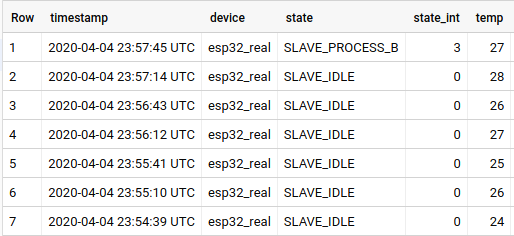
\includegraphics[width=\textwidth]{./Figures/gcloud_big_query.png}
\caption{Datos obtenidos de la base de datos en Big Query.}
\label{fig:gcloud_big_query}
\end{figure}

Al estar la información almacenada en una base de datos, es posible obtener datos de casos específicos mediante consultas SQL (\emph{Structured Query Language}) \citep{sql}, lo que brinda una herramienta de análisis sumamente poderosa. Por ejemplo, con las sentencias del algoritmo 4.1 se pueden obtener todos los registros en los que el dispositivo con ID \enquote{esp32\_real} tuvo una temperatura mayor a 40 grados. Los resultados que se obtienen con la consulta se pueden observar en la figura \ref{fig:gcloud_big_query_filter}.


\begin{lstlisting}[label=sql_query:vControl,caption=Consulta SQL para obtener información de la base de datos en Big Query.]
SELECT * FROM esp32_dataset.esp32_data
WHERE device="esp32_real" AND temp > 40
ORDER BY timestamp DESC
\end{lstlisting}

\begin{figure}[h]
\centering
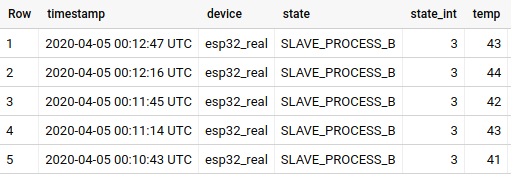
\includegraphics[width=\textwidth]{./Figures/gcloud_big_query_filter.png}
\caption{Datos obtenidos de la base de datos con la consulta del algoritmo 4.1.}
\label{fig:gcloud_big_query_filter}
\end{figure}

Además de acceder a los datos crudos, es posible obtener diferentes gráficos para analizar con mayor facilidad la información. En la figura \ref{fig:gcloud_active_devices} se puede observar el más simple de ellos, en el que se muestran los dispositivos activos a lo largo del tiempo. En este caso se utilizó un único módulo para enviar mensajes a Google Cloud, por lo tanto el número máximo de dispositivos es siempre 1. Este gráfico fue elaborado utilizando el servicio de \emph{Monitoring}, ofrecido también por la propia plataforma, y que permite monitorear prácticamente cualquier recurso que se utilice.

\begin{figure}[h]
\centering
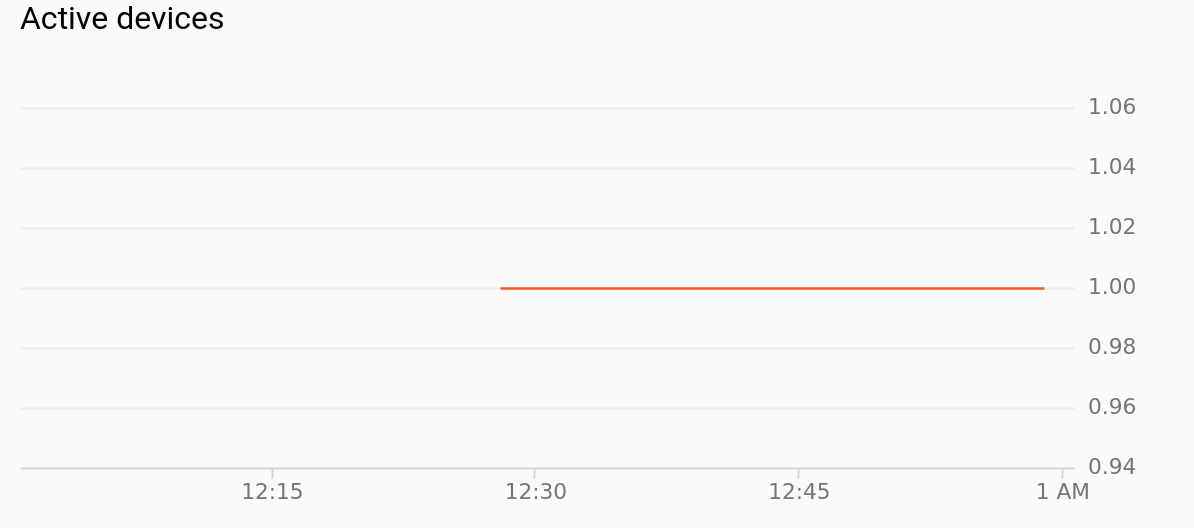
\includegraphics[width=\textwidth]{./Figures/gcloud_active_devices.png}
\caption{Gráfico con los dispositivos activos a lo largo del tiempo.}
\label{fig:gcloud_active_devices}
\end{figure}

Las figuras \ref{fig:gcloud_publish_operations} y \ref{fig:gcloud_bytes_sent} muestran otros gráficos que el servicio de \emph{Monitoring} permite efectuar. En el primer caso se grafica la cantidad total de operaciones de publicación de mensajes a lo largo del tiempo. En el segundo caso se muestra la cantidad total de bytes de información enviados desde los dispositivos hacia Google Cloud, lo cual permite tener una noción exacta del ancho de banda que se está utilizando.

\begin{figure}[h]
\centering
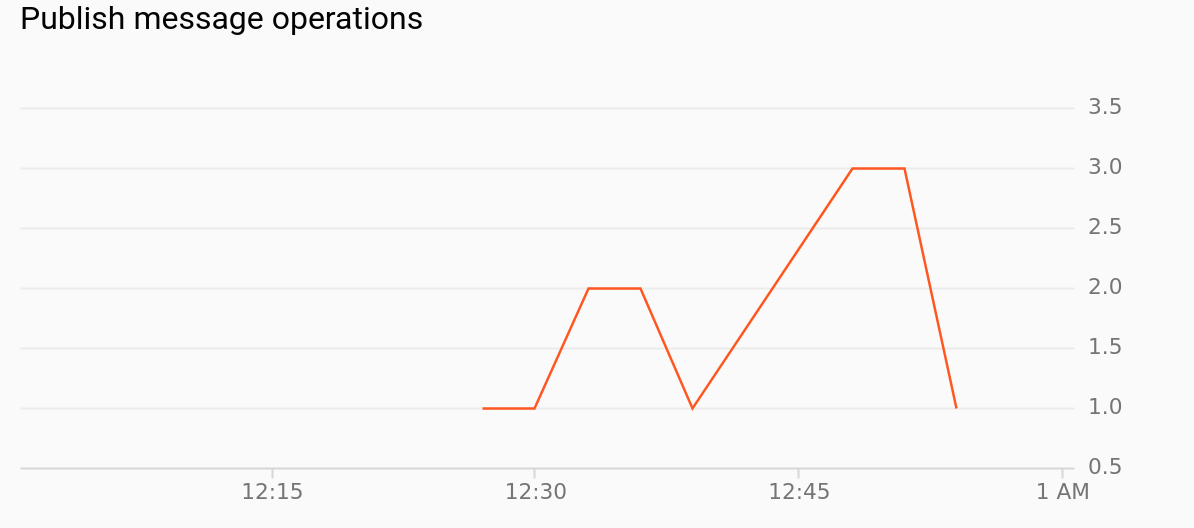
\includegraphics[width=\textwidth]{./Figures/gcloud_publish_operations.png}
\caption{Gráfico con la cantidad de operaciones de publicación de mensajes a lo largo del tiempo.}
\label{fig:gcloud_publish_operations}
\end{figure}

\begin{figure}[h]
\centering
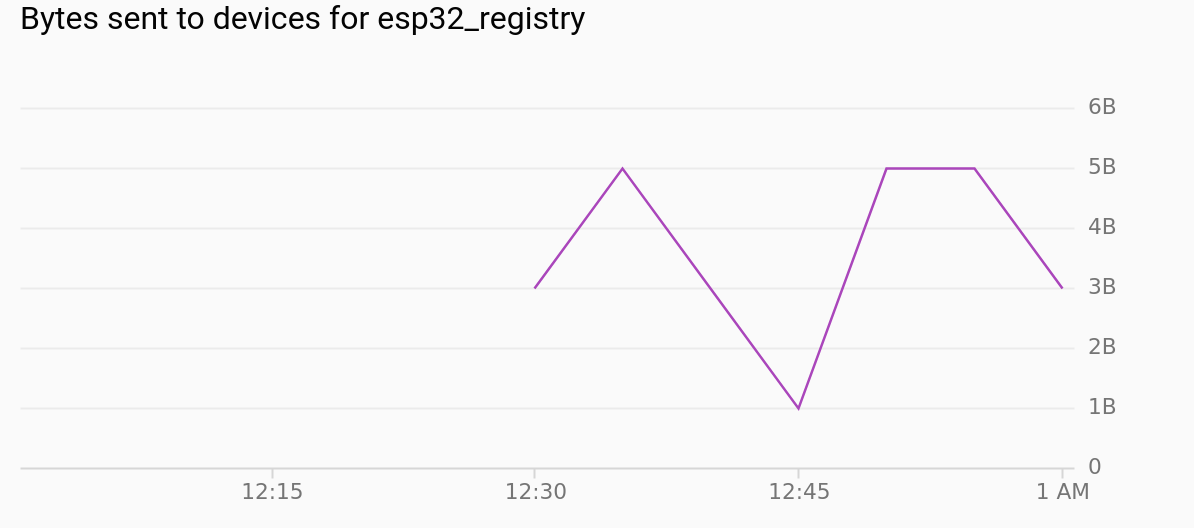
\includegraphics[width=\textwidth]{./Figures/gcloud_bytes_sent.png}
\caption{Gráfico con la cantidad de bytes de información enviados a Google Cloud.}
\label{fig:gcloud_bytes_sent}
\end{figure}

Finalmente, para completar el flujo de la arquitectura implementada en Google Cloud Platform, la información almacenada en Big Query se puede utilizar como fuente de datos para Grafana, permitiendo confeccionar gráficos personalizados para visualizar las variables de interés. La versatilidad en los gráficos que se pueden elaborar es muy amplia, ya que para determinar los datos a mostrar se utilizan consultas SQL que permiten filtrar entradas de la base de datos con facilidad.

En la figura \ref{fig:gcloud_grafana} se muestra un gráfico que se elaboró utilizando Grafana, en el que se grafica la temperatura reportada por el microcontrolador a lo largo del tiempo. Se hace una distinción de los valores reportados de acuerdo al estado del electrodoméstico en ese momento (color verde para las temperaturas estando en SLAVE\_IDLE y color naranja para el estado SLAVE\_PROCESS\_B), lo cual posibilitaría encontrar una relación entre la temperatura y el estado del dispositivo. También se muestran los valores mínimo, máximo, promedio y actual (el último medido) para cada estado. Además, en el gráfico se traza un limite en una temperatura de 40 grados (la zona roja del gráfico), para poder visualizar fácilmente los puntos que superen ese umbral.

\begin{figure}[h]
\centering
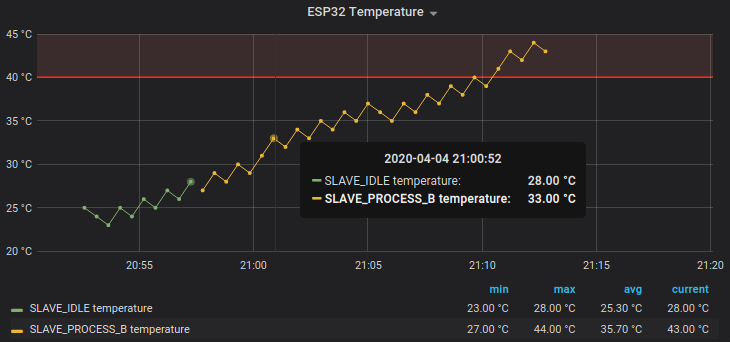
\includegraphics[width=\textwidth]{./Figures/gcloud_grafana.png}
\caption{Gráfico elaborado con Grafana a partir de los datos almacenados en la base de datos de Big Query.}
\label{fig:gcloud_grafana}
\end{figure}

El verdadero potencial de Google Cloud se puede aprovechar cuando se tienen múltiples dispositivos conectados enviando datos, pero en este caso solamente se cuenta con un único módulo de hardware para publicar información. Para solventar esta problemática, se utilizó un \emph{script} en Python para simular dispositivos adicionales conectados, publicando mensajes periódicamente de la misma forma que lo haría un electrodoméstico real. Así se obtiene el gráfico de la figura \ref{fig:gcloud_grafana_multiple}, en el que se muestran múltiples dispositivos en simultáneo a lo largo del tiempo.

\begin{figure}[h]
\centering
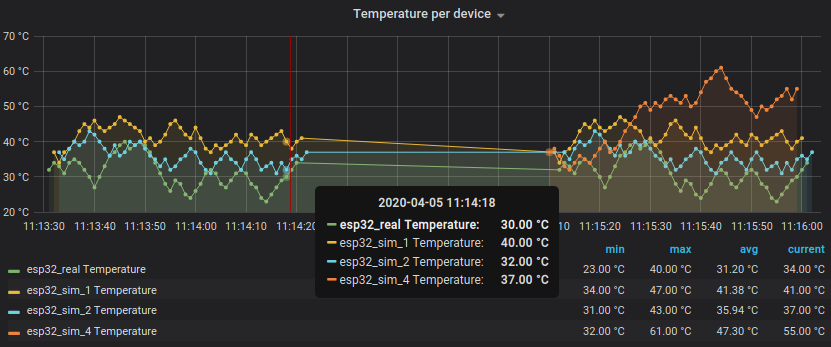
\includegraphics[width=\textwidth]{./Figures/gcloud_grafana_multiple.png}
\caption{Gráfico elaborado con Grafana a partir de los datos en Big Query de varios dispositivos.}
\label{fig:gcloud_grafana_multiple}
\end{figure}



